\documentclass[runningheads]{llncs}

\usepackage{tikz}
\usepackage{tikz-qtree}
\usepackage{graphicx}
\usepackage{amsmath}
\usepackage{mathtools}
\usepackage{array}
\usepackage{algorithm}
\usepackage[noend]{algpseudocode}
\usepackage{graphicx}
\graphicspath{{./}}

\begin{document}

% \thanks{Supported by organization x.}
\title{Semantic Genetic Programming on the GPU}
\author{João David\inst{1} \and
Ye Yang\inst{1}
}
%\authorrunning{F. Author et al.}

\institute{Departamento de Informática da Faculdade de Ciências da Universidade de Lisboa
\email{\{fc49448,fc49521\}@alunos.fc.ul.pt}}

\maketitle

\begin{abstract}
Semantic Genetic programming aims to not only syntatically manipulate the data to promote a better fitness test, but also ensuring that the resulting function is semantically correct. Traditional implementations of genetic programs have always been done on CPU, taking advantage of its multiple cores to do parallel work. We aim to improve on the parallelization of the algorithm by implementing on the Graphics Processing Unit (GPU), taking advantage of its vast amount of processing cores, which are multiple times that of the CPU. The implementation will be done on an NVidia GPU which allows us to use the supported Compute Unified Device Architecture (CUDA) API, which allows us to directly manipulate the GPU memory and threads necessary to perform fitness tests and crossover.

\keywords{Semantic Genetic programming  \and GPU \and CUDA.}
\end{abstract}
%
%
%
\section{Introduction}


The introduction should set the context for your project. Why is this topic relevant?

You should also define the scope of your project. You could design a software artifact that would end poverty and famine, but that is not realistic.

For example, this document describes the structure your paper should have. Despite using the LNCS LaTeX template \footnote{LNCS is the official template for Europar 2019, in case you are interested.}, the formatting template is not relevant, only the content structure is relevant.

Finally, you should define the goals of your project. For instance,

\begin{itemize}
	\item To propose a method for the parallelization of Genetic Algorithms
	\item An implementation of such algorithm
	\item The experimental evaluation of such method, with comparison with a sequential alternative.
\end{itemize}


\section{Background}
To understand the underlying principles of the implementation we first have to introduce the main concepts.
\begin{itemize}
	\item The semantic syntax our work will be based on will be presented as a tree structure, each node containing either a mathematical operator, a constant or a variable which can be swapped by a value from a given data set.
	\item To start off the program, we must introduce an initial data set. The data set will be read as a text file, each line of the text file containing randomly generated values and a final target value. These random data set values are to be added to trees that contain variables, each variable having its own index to determine which random value to swap the variable by. After all the necessary swaps are made, the final value is computed for each line of the data set and the fitness of the syntax tree is determined by calculating the Mean Squared Error (MSE) between the calculated values (O) and the target values (T): $$\frac{1}{n}\sum_{i=1}^{n} (O_i - T_i)^{2}$$
\end{itemize}

The main parallelization applied to the algorithm is done by taking advantage of the much higher amount of threads on a GPU compared to a CPU. In order to better take advantage of all the computational power on the GPU we first have to copy all the data from CPU memory to GPU memory by allocating memory for the array using cudaMalloc(\texttt{t\_array,size}) and then copying the data currently residing on CPU memory to the newly GPU memory allocated array using cudaMemcpy(\texttt{o\_array,t\_array,size,cudaMemcpyHostToDevice}). The keyword cudaMemcpyHostToDevice signals that the array from which the contents are to be copied (\texttt{o\_array}) is residing in CPU memory and the target array to which the values are copied to (\texttt{t\_array}) is residing in the GPU memory. These are ncessary steps since neither the GPU nor the CPU have direct access to each other's memory region.

\section{Approach}
The main genetic algorithm to crossover different trees of computation takes into account the following variables:
\begin{itemize}
	\item \textit{N} $\rightarrow$ \ the total number of trees
	\item \textit{gen} $\rightarrow$ \ the current generation cycle
	\item \textit{threadId} $\rightarrow$ \ the ID of a GPU thread
\end{itemize}

Each node on a syntax can hold a literal value, a variable or a mathematical operation. When processing a tree through a data set, each variable will be swapped by the corresponding value in the data set according to the variables index. In Figure \ref{syntree} we can see the tree representation of the mathematical formula $x0 * (x1+4)$ which is then processed according to a data set line containing the values: $0.5\quad 25.3\quad 6.2\quad 12$\ . The values within the data set that are not referenced by any variable in the tree are ignored, the final value computed is compared with the target value (12) which will evaluate the fitness of the tree.

\begin{figure}
\hfil
\begin{tikzpicture}
  \Tree [.* [.x0 ] 
             [.+ [.x1 ] [.4 ]]]
  %
  \begin{scope}[shift = {(5cm, 0cm)}]
  \Tree [.* [.$0.5$ ]  
            [.+ [.$25.3$ ] [.4 ]]]
  \end{scope}
  %
  \draw[->, yshift = -1.5cm] (2, 0) -- (3, 0);
\end{tikzpicture}
\hfil
\caption{Syntax tree value swap example}
\label{syntree}
\end{figure}

Given the initial data set, we first have to run the values through all the generated trees, after which we compute the respective fitness values for every single tree and store it in a matrix. We then place the indexes of each tree in the first row of a $N * gen$ sized matrix. Each column represents a concatenation of trees by summation, the trees are represented by their indexes from 0 to N-1.

The algorithm works as follows: for every even generation cycle, the GPU threads with even IDs will look for the best fitness only within the even numbered indexes on the matrix. The GPU threads with odd numbered IDs will do the same but on odd indexes. When the best fitness is found, the index of the column to which it belongs will be appended to that generation cycle (or row).

For every odd generation cycle, the GPU threads within the first half of the X axis in the tree index matrix will look for the best fitness within the first half of the matrix, the rest of the threads will search the other half. To each half of the row of the current generation cycle, the index of best fitness of the respective half will be appended.

Given this alternating crossover algorithm, we can achieve a less linear evolution from generation to generation of each sequence. At Algorithm~\ref{crossover_alg} we can see a pseudo code representation of the algorithm.

\begin{algorithm}
\caption{Tree crossover}
\begin{algorithmic}[1]
\Procedure{TreeCrossover}{}
\State \textbf{int} \textit{max}
\If {$\textit{gen} \ \%\ 2 == 0$} 
	\For{$i = threadId\ \%\ 2;\ i < N;\ i+=2$}
		\State {find highest fitness and store in \textit{max}}
	\EndFor
\Else \If {$threadId \ < N/2$}
	\For{$i = 0;\ i < N/2;\ i++$}
		\State {find highest fitness and store in \textit{max}}
	\EndFor
\Else
	\For{$i = N/2;\ i < N;\ i++$}
		\State {find highest fitness and store in \textit{max}}
	\EndFor
\EndIf
\EndIf
\State \Return \textit{max}
\EndProcedure
\end{algorithmic}
\label{crossover_alg}
\end{algorithm}


\section{Implementation Details}
Before any values could be first calculated, we needed some form of input to compare values with. This lead to the implementation of a data set parser. The data set is a text file in which all the variables and target values are defined. Each line has an equal amount of values \textit{Y} written, the last of which corresponds to the target value. Both variable values and target values are then extracted and stored in separate arrays which will be used to calculate the fitness for the first generation of trees.

To store and calculate the values, a set number of random syntax trees have to be initially generated. Each node of the tree as previously mentioned can be a literal value, a variable or a mathematical operator. After generating the trees, each one of them must be run through the data set to evaluate its fitness by calculating the mathematical operations defined and comparing it with the target values. The computation is handled as a Reverse Polish Notation calculator (RPN) according to the following procedures:
\begin{itemize}
	\item A seperate LIFO stack to store literal values and variables is created
	\item The tree is traversed in postorder so that the root operation or value is read last
	\item If either a literal or a variable are present, they are pushed into the stack
	\item If a mathematical operation is read, 2 values are popped out of the stack for computing, and the resulting value is pushed back into the stack
	\item At the end of the processing, the final value is popped from the stack and stored in a result matrix of size $$N_{trees}*dataset_{rows}$$ with each row representing the calculated values for a given data set row by a syntax tree and each column the resulting values to compare with the target values.
\end{itemize}

\subsection{GPU Parallelization}
After all the values are calculated and stored in the array, we then proceed to the computation of the fitness for all trees on the first generation. In Figure~\ref{fitness_calc} we present an example of fitness calculation with a data set of 4 lines, meaning that each tree computes 4 different values which are compared to the 4 target values to determine the MSE and consequently the fitness of the tree. Each tree is processed by a block (an abstract representation of a group of executing threads) which will have its own ID that can be extracted with the built in keyword \textit{blockIdx.x}. The \textit{.x} termination means we are extracting the ID along the \textit{x} axis, since the kernel is launched in 1 dimension, both the \textit{y} and \textit{z} values are 0.

$V_{i,j}$ is the value calculated by a tree of ID \textit{i} on line \textit{j} of the data set and $T_{j}$ the respective target value. Each $(V_{i,j} - T_{j})^{2}$ value is calculated by a single thread which is able to compute the correct index on the array by calculating its position relative to its own ID (\textit{threadIdx.x}) and the block's ID in the following manner: array[$(blockIdx.x * num\_rows) + threadIdx.x$].

After all values are calculated we then proceed to a reduction phase, in this phase the amount of threads working on adding up all the values is reduced by half with each step until it reaches 1, which will be the final value to be divided by \texttt{num\_rows} which will equal to the MSE of the computed value and the target value i.e. the fitness of the tree. Since all blocks work in parallel, the complexity of the reduction algorithm is $O(log(n))$.


\begin{figure}[!htb]
\begin{center}
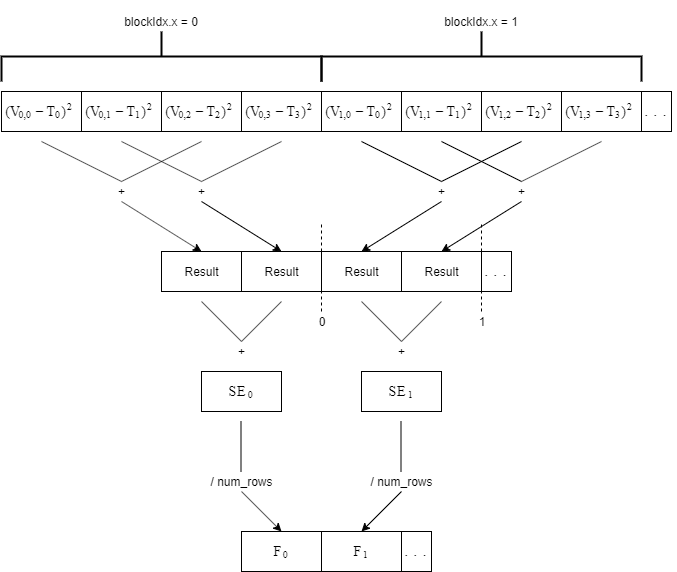
\includegraphics[scale=0.35]{Fitness_Calculation1}
\end{center}
\caption{Fitness computation for a data set of 4 lines}
\label{fitness_calc}
\end{figure}

\section{Evaluation}

\subsection{Experimental Setup}

\begin{center}
 \begin{tabular}{|>{\centering\arraybackslash}p{4cm}|>{\centering\arraybackslash}p{2cm}|>{\centering\arraybackslash}p{2cm}|>{\centering\arraybackslash}p{2cm}|} 
 \hline
 Processor & CPU Cores & Threads & RAM \\ [0.5ex] 
 \hline\hline
 Intel Xeon X5670 & 12 & 24 & 24GB \\
 \hline
\end{tabular}
\end{center}

\begin{center}
\begin{tabular}{|>{\centering\arraybackslash}p{4cm}|>{\centering\arraybackslash}p{2cm}|>{\centering\arraybackslash}p{2cm}|>{\centering\arraybackslash}p{2cm}|}
 \hline
 Graphics Card & GPU Cores & Threads & Memory \\ [0.5ex] 
 \hline\hline
 Intel Xeon X5670 & 1024 & 24 & 4GB\\  
 \hline
\end{tabular}
\end{center}

In this section you should describe the machine(s) in which you are going to evaluate your system. Select the information that is relevant.


\subsection{Results}

In this section you should present the results. Do not forget to explain where the data came from. 

You should include (ideally vectorial) plots, with a descriptive caption. Make sure all the plots (Like Figure~\ref{fig1} are well identified and axis and metrics are defined.

\subsection{Discussion}

Here you should discuss the results on a high level. For instance, based on our results, the parallelization of the merge-sort is relevant as no other parallel work occurs at the same time, and the complexity $O(Nlog(N))$ can have a large impact when the number of individuals is high.

\section{Related Work}

Alberto Moraglio, Krzysztof Krawiec, and Colin G. Johnson introduced a new way of genetic programming, Geometric Semantic Genetic Programming (GSGP) which consists in changing the semantics of the functions directly. Their work in regards to fitness evaluation, tree mutation and crossover is far more complex given that we only accounted for mutation by concatenation with sums of trees. However the implementation of the genetic algorithm was done on CPU which makes performance considerably slower if it were implemented on GPU.


\section{Conclusions}

Here you should resume the major conclusions taken from discussion. Ideally, these should align with the objectives introduced in the introduction.


You should also list the future work, i. e., tasks and challenges that were outside your scope, but are relevant.

\section*{Acknowledgements}

First Author wrote the part of the program implemented the phasers. Second Author implemented the MergeSort in parallel. 

Both authors wrote this paper, with First Author focusing on the introduction, related work and conclusions while the Second Author focused on approach and evaluation.

Each author spent around 30 hours on this project.

\bibliographystyle{splncs04}
\bibliography{bibliography}

\end{document}
